\chapter{Probability and Statistics}
\label{chap:Probability and Statistics}
One role for the distributions is to model the probability distribution $p(\vec{x})$ of a random variable $x$,given a finite set of observations.This problem is known as \textbf{density estimation}.We shall assume that the data points are independent and identically distributed.

\textbf{Parameter} distributions are governed by a small number of adaptive parameters,such as the mean and variance in the case of a Gaussian for example.In a frequentist treatment, we choose specific values for the parameters by optimizing some criterion, such as the likelihood function. By contrast, in a Bayesian treatment we introduce prior distributions over the parameters and then use Bayes’ theorem to compute the corresponding posterior distribution given the observed data.

An important role is played by \textbf{conjugate priors},that lead to posterior distributions having the same functional form as the prior,and that therefore lead to a greatly simplified Bayesian analytics.

\textbf{Nonparametric} density estimation methods in which the form of the distribution typically depends on the size of the data set.Parameters in such models control the model complexity rather than the form of the distribution.We cover three nonparametric methods based respectively on histograms,nearest-neighbours,and kernels.

\section{Frequentists vs. Bayesians}
There are two different interpretations of probability.
One is called the \textbf{frequentist} interpretation. In this view, probabilities represent long run \textbf{frequencies} of events. For example, the above statement means that, if we flip the coin many times, we expect it to land heads about half the time.

The other interpretation is called the \textbf{Bayesian} interpretation of probability. In this view, probability is used to quantify our \textbf{uncertainty} about something; hence it is fundamentally related to information rather than repeated trials (Jaynes 2003). In the Bayesian view, the above statement means we believe the coin is equally likely to land heads or tails on the next toss

One big advantage of the Bayesian interpretation is that it can be used to model our uncertainty about events that do not have long term frequencies. For example, we might want to compute the probability that the polar ice cap will melt by 2020 CE. This event will happen zero or one times, but cannot happen repeatedly. Nevertheless,we thought to be able to quantify our uncertainty about this event. To give another machine learning oriented example, we might have observed a “blip” on our radar screen, and want to compute the
probability distribution over the location of the corresponding target (be it a bird, plane, or missile). In all these cases, the idea of repeated trials does not make sense, but the Bayesian interpretation is valid and indeed quite natural. We shall therefore adopt the Bayesian interpretation in this book. Fortunately, the
basic rules of probability theory are the same, no matter which interpretation is adopted.


\section{probability theory}

%\subsection{Basic concepts}
\subsection{Concepts}
The expression $p(A)$ denotes the probability that event A is true.We require that $0\leq p(A) \leq 1$,where 0 means the event definitely will not happen,and $p(A)=1$ means the event definitely will happen.$p(\hat{A})$ denotes the probability of the event not A;this is defined to be $p(\hat{A})=1-p(A)$.

We denote a random event by defining a \textbf{random variable} $X$.

\textbf{Descrete random variable}: $X$ ,which can take on any value from a finite or countably infinite set .We denote the probability of the event that $X=x$ by $p(X=x)$,or just $p(x)$ for short.Here $p()$ is called a \textbf{probability mass function} or \textbf{pmf}.The pmfs are defined one \textbf{state space}.$\mathbb{I}$ denotes the binary \textbf{indicator funcition}.

\textbf{Continuous random variable}: the value of $X$ is real-valued.

\textbf{prior probability distribution}
In Bayesian statistical inference, a prior probability distribution, often called simply the prior, of an uncertain quantity p is the probability distribution that would express one's uncertainty about p \textbf{before} some evidence is taken into account.

\textbf{posterior probability distribution}
In Bayesian statistics, the posterior probability of a random event or an uncertain proposition is the conditional probability that is assigned \textbf{after} the relevant evidence or background is taken into account.

\textbf{likelihood function}
In statistics, a likelihood function (often simply the likelihood) is a function of the parameters of a statistical model.The likelihood of a set of parameter values, θ, given outcomes x, is equal to the probability of those observed outcomes given those parameter values

\subsection{Fundamental rules}
In this section,we review the basic rule of probability.
\subsubsection{Probability of a union of two events}
Given two events,$A$ and B,we define the probability of A or B as follows:
\begin{align}
p(A\cup B)& = p(A) + p(B) - p(A\cap B)	\\
		  & = p(A) + p(B)
\end{align}
if A and B are mutually independent 


\subsubsection{Joint probabilities}
We define the probability of the joint event A and B as follows:
\begin{equation}
p(A,B) = p(A\cap B) = p(A|B)p(B)
\end{equation}
This is sometimes called the \textbf{product rule}
\subsubsection{Conditional probability}
Define the \textbf{conditional probability} of event A,given that event B is true,as follows:
\begin{equation}
p(A|B)= \frac{p(A,B)}{p(B)},if p(B) > 0
\end{equation}
\subsubsection{CDF}

\begin{equation}
F(x) \triangleq P(X \leq x)=\begin{cases}
\sum_{u \leq x}p(u) & \text{, discrete}\\
\int_{-\infty}^{x} f(u)\mathrm{d}u & \text{, continuous}\\
\end{cases}
\end{equation}


\subsubsection{PMF and PDF}
For descrete random variable, We denote the probability of the event that $X=x$ by $P(X=x)$, or just $p(x)$ for short. Here $p(x)$ is called a \textbf{probability mass function} or \textbf{PMF}.A probability mass function is a function that gives the probability that a discrete random variable is exactly equal to some value\footnote{\url{http://en.wikipedia.org/wiki/Probability_mass_function}}. This satisfies the properties $0 \leq p(x) \leq 1$ and $\sum_{x \in \mathcal{X}} p(x)=1$.

For continuous variable, in the equation $F(x)=\int_{-\infty}^{x} f(u)\mathrm{d}u$, the function $f(x)$ is called a \textbf{probability density function} or \textbf{PDF}. A probability density function is a function that describes the relative likelihood for this random variable to take on a given value\footnote{\url{http://en.wikipedia.org/wiki/Probability_density_function}}.This satisfies the properties $f(x) \geq 0$ and $\int_{-\infty}^{\infty} f(x)\mathrm{d}x=1$.


\subsection{Mutivariate random variables}


\subsubsection{Joint CDF}
We denote joint CDF by $F(x,y) \triangleq P(X \leq x \cap Y \leq y)=P(X \leq x , Y \leq y)$.

\begin{equation}
F(x,y) \triangleq P(X \leq x, Y \leq y)=\begin{cases}
\sum_{u \leq x, v \leq y}p(u,v) \\
\int_{-\infty}^{x}\int_{-\infty}^{y} f(u,v)\mathrm{d}u\mathrm{d}v \\
\end{cases}
\end{equation}

\textbf{product rule}:
\begin{equation}\label{eqn:product-rule}
p(X,Y)=P(X|Y)P(Y)
\end{equation}

\textbf{Chain rule}:
\begin{equation}
p(X_{1:N})=p(X_1)p(X_3|X_2,X_1)...p(X_N|X_{1:N-1})
\end{equation}


\subsubsection{Marginal distribution}
\textbf{Marginal CDF}:
\begin{equation}\begin{split}
F_X(x) \triangleq F(x,+\infty)= 
& \begin{cases}
\sum\limits_{x_i \leq x}P(X=x_i)=\sum\limits_{x_i \leq x}\sum\limits_{j=1}^{+\infty}P(X=x_i,Y=y_j) \\
\int_{-\infty}^{x}f_X(u)du=\int_{-\infty}^{x}\int_{-\infty}^{+\infty} f(u,v)\mathrm{d}u\mathrm{d}v \\
\end{cases}
\end{split}\end{equation}

\begin{equation}\begin{split}
F_Y(y) \triangleq F(+\infty,y)= 
& \begin{cases}
\sum\limits_{y_j \leq y}p(Y=y_j)=\sum\limits_{i=1}^{+\infty}\sum_{y_j \leq y}P(X=x_i,Y=y_j) \\
\int_{-\infty}^{y}f_Y(v)dv=\int_{-\infty}^{+\infty}\int_{-\infty}^{y} f(u,v)\mathrm{d}u\mathrm{d}v \\
\end{cases}
\end{split}\end{equation}

\textbf{Marginal PMF and PDF}:
\begin{equation} \begin{cases}
P(X=x_i)=\sum_{j=1}^{+\infty}P(X=x_i,Y=y_j) & \text{, descrete}\\
f_X(x)=\int_{-\infty}^{+\infty} f(x,y)\mathrm{d}y & \text{, continuous}\\
\end{cases}\end{equation}

\begin{equation}\begin{cases}
p(Y=y_j)=\sum_{i=1}^{+\infty}P(X=x_i,Y=y_j) & \text{, descrete}\\
f_Y(y)=\int_{-\infty}^{+\infty} f(x,y)\mathrm{d}x & \text{, continuous}\\
\end{cases}\end{equation}


\subsubsection{Conditional distribution}
\textbf{Conditional PMF}:
\begin{equation}
p(X=x_i|Y=y_j)=\dfrac{p(X=x_i,Y=y_j)}{p(Y=y_j)} \text{ if } p(Y)>0
\end{equation}
The pmf $p(X|Y)$ is called \textbf{conditional probability}.

\textbf{Conditional PDF}:
\begin{equation}
f_{X|Y}(x|y)=\dfrac{f(x,y)}{f_Y(y)}
\end{equation}

\subsection{Bayes rule}
\begin{equation}
\begin{split}
p(Y=y|X=x) & =\dfrac{p(X=x,Y=y)}{p(X=x)} \\
           & =\dfrac{p(X=x|Y=y)p(Y=y)}{\sum_{y'}p(X=x|Y=y')p(Y=y')}
\end{split}
\end{equation}

sum rule
\begin{equation}
                                  p(X) = \sum_{Y}p(X,Y)
\end{equation}
product rule
\begin{equation}
                                  p(X,Y) = p(Y|X)p(X)
\end{equation}
Bayes' theorem
\begin{equation}
                                  p(Y|X) = \frac{p(X|Y)p(Y)}{p(X)}
\end{equation}
Denominator in Bayes' theorem
\begin{equation}
                                  p(X) = \sum_Y{p(X|Y)p(Y)}
\end{equation}
probability densities
\begin{equation}
                         p(x\in (a,b)) = \int_{a}^{b}p(x)dx
\end{equation}
The probability density function p(x) must satisfy the two conditions
\begin{equation}
\begin{cases}
                                  p(x) \geq 0               \\
                                  \int_{-\infty}^{\infty}p(x)dx = 1
\end{cases}
\end{equation}

Combinations of discrete and continuous variables.
\begin{equation}
                                  p(x) = \int_p(x,y)dy	
\end{equation}
\begin{equation}
                                  p(x,y) = p(y|x)p(x)
\end{equation}


Bayesian probabilities
So far, we have viewed probabilities in terms of the frequencies of random,repeatable events,which we shall refer to as the classical or frequentist interpretation of probability.Now we turn to the more general Bayesian view,in which probabilities provide a quantification of uncertainty.

We can adopt a similar approach when making inferences about quantities such as the parameters $\mathbf{w}$ in the polynomial curve fitting.We capture our assumptions about \textbf{w},before observing the data,in the form of a \textbf{prior} probability distribution $p(\mathbf{w})$.The effect of the observed data $\mathcal{D} = {t_1,...,t_N}$ is expressed through the conditional probability $p(D|w)$.Bayes' theorem,which takes the form
\begin{equation}
p(\textbf{w}|\mathcal{D}) = \frac{p(\mathcal{D}|\textbf{w})p(\textbf{w})}{p(\mathcal{D})}
\end{equation}
then allows us to evaluate the uncertainty in $\vec{w}$ \textbf{after} we have observed $\mathcal{D}$ in the form of the \textbf{posterior} probability $p(\mathbf{w}|\mathcal{D})$.

The quantity $p(D|w)$ on the right-hand side of Bayes' theorem is evaluated for the observed data set D and 
can be viewed as a function of the parameter vector $\mathbf{w}$,in which case it is called the \textbf{likelihood function}.It expresses how probable the observed data set is for different settings of the parameter vector $\vec{w}$.
\begin{equation}
posteroir \propto likelihood \times prior
\end{equation}
where all of these quantities are viewed as functions of $\vec{w}$.
 Integrating both side with respect to $\mathbf{w}$
 \begin{equation}
p(D) = \int p(D|\mathbf{w}) p(\mathbf{w})d\mathbf{w} 
 \end{equation}

A widely used frequentist estimator is \textbf{maximum likelihood},in which $\mathbf{w}$ is set to the value that maximizes the likelihood function $p(\mathcal{D}|w)$.In the machine learning literature,the negative log of the likelihood function is called an \textbf{error function}.

Oner approach to determining the frequentist error bars is the \textbf{bootstrap},in which multiple data sets are created as follows.Suppose out original data set consists of $N$ data points.We can create a new data set $X_B$ by drawing $N$ points at random from $X$, with \textbf{replacement}, so that some points in X may be replicated in XB, whereas other points in X may be absent from $X_B$. This process can be repeated L times to generate L data sets each of size N and each obtained by sampling from the original data set X. The statistical accuracy of parameter estimates can then be evaluated by looking at the variability of predictions between the different bootstrap data sets.



\subsection{Independence and conditional independence}
We say $X$ and $Y$ are unconditionally independent or marginally independent, denoted $X \perp Y$, if we can represent the joint as the product of the two marginals, i.e.,
\begin{equation}
X \perp Y=P(X,Y)=P(X)P(Y)
\end{equation}

We say $X$ and $Y$ are conditionally independent(CI) given $Z$ if the conditional joint can be written as a product of conditional marginals:
\begin{equation}
X \perp Y|Z=P(X,Y|Z)=P(X|Z)P(Y|Z)
\end{equation}

\subsection{Quantiles}
Since the cdf $F$ is a monotonically increasing function, it has an inverse; let us denote this by $F^{-1}$. If $F$ is the cdf of $X$ , then $F^{-1}(\alpha)$ is the value of $x_{\alpha}$ such that $P(X \leq x_{\alpha})=\alpha$; this is called the $\alpha$ quantile of $F$. The value $F^{-1}(0.5)$ is the \textbf{median} of the distribution, with half of the probability mass on the left, and half on the right. The values $F^{-1}(0.25)$ and $F^{−1}(0.75)$are the lower and upper \textbf{quartiles}.

\subsection{Mean and variance}
The most familiar property of a distribution is its \textbf{mean},or \textbf{expected value}, denoted by $\mu$. For discrete rv’s, it is defined as $\mathbb{E}[X] \triangleq \sum_{x \in \mathcal{X}}xp(x)$, and for continuous rv’s, it is defined as $\mathbb{E}[X] \triangleq \int_{\mathcal{X}}xp(x)\mathrm{d}x$. If this integral is not finite, the mean is not defined (we will see some examples of this later). 

The \textbf{variance} is a measure of the “spread” of a distribution, denoted by $\sigma^2$. This is defined as follows:
\begin{align}
var[X]& =\mathbb{E}[(X-\mu)^2] \\
      & =\int{(x-\mu)^2p(x)\mathrm{d}x} \nonumber \\
      & =\int{x^2p(x)\mathrm{d}x}+{\mu}^2\int{p(x)\mathrm{d}x}-2\mu\int{xp(x)\mathrm{d}x} \nonumber \\
	  & =\mathbb{E}[X^2]-{\mu}^2
\end{align}

from which we derive the useful result
\begin{equation}
\mathbb{E}[X^2]=\sigma^2+{\mu}^2
\end{equation}

The \textbf{standard deviation} is defined as
\begin{equation}
std[X] \triangleq \sqrt{var[X]}
\end{equation}

This is useful since it has the same units as $X$ itself.

Expectations and covariances
The average value of some function $f(x)$ under a probability distribution p(x) is called the expectation of f(x) and
will be denoted by 
\begin{equation}
                                  \mathbb{E}[f] = \sum_{x}p(x)f(x)
                                  \mathbb{E}[f] = \int p(x)f(x)dx
\end{equation}

approximation
\begin{equation}
\mathbb{E}[f] \simeq \frac{1}{N}\sum_{n=1}^{N}{f(x_n)}
\end{equation}
                                  
conditional expectation with respect to a conditional distribution                                
\begin{equation}
\mathbb{E}_x[f|y] = \sum_{x}p(x|y)f(x)
\end{equation}

variance of f(x) is defined by
\begin{equation}
var[f] = \mathbb{E}[(f(x) - \mathbb{E}[f(x)])^2
var[f] = \mathbb{E}[f(x)^2]-\mathbb{E}[f(x)]^2
\end{equation}
convariance 
\begin{equation}
cov[x,y] = \mathbb{E}_{x,y}[\{x- \mathbb{E}[x]\}\{y-\mathbb{E}[y]\}]
\end{equation}

In the case of two vectors of random variables \textbf{x} and \textbf{y}
\begin{equation}
cov[\textbf{x},\textbf{y}] = \mathbb{E}_{x,y}[\{\textbf{x}-\mathbb{E}[\textbf{x}]\} \{ \textbf{y}^T - \mathbb{E}[\textbf{y}^T ]\}] \\
cov[\textbf{x},\textbf{y}] = \mathbb{E}_{x,y}[\textbf{x}\textbf{y}^T] - \mathbb{E}[\textbf{x}] \mathbb{E}[\textbf{y}^T]
\end{equation}

\section{Some common discrete distributions}
In this section, we review some commonly used parametric distributions defined on discrete state spaces, both finite and countably infinite.


\subsection{The Bernoulli and binomial distributions}

\begin{definition}
Now suppose we toss a coin only once. Let $X \in \{0,1\}$ be a binary random variable, with probability of “success” or “heads” of $\theta$. We say that $X$ has a \textbf{Bernoulli distribution}. This is written as $X \sim \text{Ber}(\theta)$, where the pmf is defined as 
\begin{equation}
\text{Ber}(x|\theta) \triangleq \theta^{\mathbb{I}(x=1)}(1-\theta)^{\mathbb{I}(x=0)}
\end{equation}
\end{definition}


\begin{definition}
Suppose we toss a coin $n$ times. Let $X \in \{0,1,\cdots,n\}$ be the number of heads. If the probability of heads is $\theta$, then we say $X$ has a \textbf{binomial distribution}, written as $X \sim \text{Bin}(n, \theta)$. The pmf is given by 
\begin{equation}\label{eqn:binomial-pmf}
\text{Bin}(k|n,\theta) \triangleq \dbinom{n}{k}\theta^k(1-\theta)^{n-k}
\end{equation}
\end{definition}


\subsection{The multinoulli and multinomial distributions}

\begin{definition}
The Bernoulli distribution can be used to model the outcome of one coin tosses. To model the outcome of tossing a K-sided dice, let $\vec{x} =(\mathbb{I}(x=1),\cdots,\mathbb{I}(x=K)) \in \{0,1\}^K$ be a random vector(this is called \textbf{dummy encoding} or \textbf{one-hot encoding}), then we say $X$ has a \textbf{multinoulli distribution}(or \textbf{categorical distribution}), written as $X \sim \text{Cat}(\theta)$. The pmf is given by: 
\begin{equation}
p(\vec{x}) \triangleq \prod\limits_{k=1}^K\theta_k^{\mathbb{I}(x_k=1)}
\end{equation}
\end{definition}

\begin{definition}
Suppose we toss a K-sided dice $n$ times. Let $\vec{x} =(x_1,x_2,\cdots,x_K) \in \{0,1,\cdots,n\}^K$ be a random vector, where $x_j$ is the number of times side $j$ of the dice occurs, then we say $X$ has a \textbf{multinomial distribution}, written as $X \sim \text{Mu}(n, \vec{\theta})$. The pmf is given by 
\begin{equation}\label{eqn:multinomial-pmf}
p(\vec{x}) \triangleq \dbinom{n}{x_1 \cdots x_k} \prod\limits_{k=1}^K\theta_k^{x_k}
\end{equation}
where $\dbinom{n}{x_1 \cdots x_k} \triangleq \dfrac{n!}{x_1!x_2! \cdots x_K!}$
\end{definition}

Bernoulli distribution is just a special case of a Binomial distribution with $n=1$, and so is multinoulli distribution as to multinomial distribution. See Table \ref{tab:multinomial-summary} for a summary.

\begin{table}
\caption{Summary of the multinomial and related distributions.}
\label{tab:multinomial-summary}
\centering
\begin{tabular}{llll}
\hline\noalign{\smallskip}
Name & K & n & X \\
\noalign{\smallskip}\svhline\noalign{\smallskip}
Bernoulli & 1 & 1 & $x \in \{0,1\}$ \\
Binomial & 1 & - & $\vec{x} \in \{0,1,\cdots,n\}$ \\
Multinoulli & - & 1 & $\vec{x} \in \{0,1\}^K, \sum_{k=1}^K x_k=1$ \\
Multinomial & - & - & $\vec{x} \in \{0,1,\cdots,n\}^K, \sum_{k=1}^K x_k=n$ \\
\noalign{\smallskip}\hline
\end{tabular}
\end{table} 


\subsection{The Poisson distribution}
\begin{definition}
We say that $X \in \{0,1,2,\cdots\}$ has a \textbf{Poisson distribution} with parameter $\lambda>0$, written as $X \sim \text{Poi}(\lambda)$, if its pmf is
\begin{equation}
p(x|\lambda)=e^{-\lambda}\dfrac{\lambda^x}{x!}
\end{equation}
\end{definition}

The first term is just the normalization constant, required to ensure the distribution sums to 1.

The Poisson distribution is often used as a model for counts of rare events like radioactive decay and traffic accidents. 

\begin{table*}
\caption{Summary of Bernoulli, binomial multinoulli and multinomial distributions.}
\label{tab:Summary-distribution}
\centering
\begin{tabular}{llllll}
\hline\noalign{\smallskip}
Name & Written as & X & $p(x)$(or $p(\vec{x})$) & $\mathbb{E}[X]$ & $\text{var}[X]$ \\
\noalign{\smallskip}\svhline\noalign{\smallskip}
Bernoulli & $X \sim \text{Ber}(\theta)$ & $x \in \{0,1\}$ & $\theta^{\mathbb{I}(x=1)}(1-\theta)^{\mathbb{I}(x=0)}$ & $\theta$ & $\theta(1-\theta)$ \\
Binomial & $X \sim \text{Bin}(n,\theta)$ & $x \in \{0,1,\cdots,n\}$ & $\dbinom{n}{k}\theta^k(1-\theta)^{n-k}$ & $n\theta$ & $n\theta(1-\theta)$ \\
Multinoulli & $X \sim \text{Cat}(\vec{\theta})$ & $\vec{x} \in \{0,1\}^K, \sum_{k=1}^K x_k=1$ & $\prod\limits_{k=1}^K\theta_j^{\mathbb{I}(x_j=1)}$ & - & - \\
Multinomial & $X \sim \text{Mu}(n,\vec{\theta})$ & $\vec{x} \in \{0,1,\cdots,n\}^K, \sum_{k=1}^K x_k=n$ & $\dbinom{n}{x_1 \cdots x_k} \prod\limits_{k=1}^K\theta_j^{x_j}$ & - & - \\
Poisson & $X \sim \text{Poi}(\lambda)$ & $x \in \{0,1,2,\cdots\}$ & $e^{-\lambda}\dfrac{\lambda^x}{x!}$ & $\lambda$ & $\lambda$ \\
\noalign{\smallskip}\hline
\end{tabular}
\end{table*}


\subsection{The empirical distribution}
The \textbf{empirical distribution function}\footnote{\url{http://en.wikipedia.org/wiki/Empirical_distribution_function}}, or \textbf{empirical cdf}, is the cumulative distribution function associated with the empirical measure of the sample. Let $\mathcal{D}=\{x_1,x_2,\cdots,x_N\}$ be a sample set, it is defined as 
\begin{equation}
F_n(x) \triangleq \dfrac{1}{N}\sum\limits_{i=1}^N\mathbb{I}(x_i \leq x)
\end{equation}


\section{Some common continuous distributions}
In this section we present some commonly used univariate (one-dimensional) continuous probability distributions.


\subsection{Gaussian (normal) distribution}

% \begin{table}
% \caption{Summary of Gaussian distribution}
% \centering
% \begin{tabular}{cccccc}
% \hline\noalign{\smallskip}
% Name & Written as & $f(x)$ & $\mathbb{E}[X]$ & mode & $\text{var}[X]$ \\
% \noalign{\smallskip}\svhline\noalign{\smallskip}
% Gaussian distribution & $X \sim \mathcal{N}(\mu,\sigma^2)$ & $\dfrac{1}{\sqrt{2\pi}\sigma}e^{-\frac{1}{2\sigma^2}\left(x-\mu\right)^2}$ & $\mu$ & $\mu$ & $\sigma^2$ \\
% \noalign{\smallskip}\hline
% \end{tabular}
% \end{table} 

\begin{table}
\caption{Summary of Gaussian distribution.}
\centering
\begin{tabular}{cccccc}
\hline\noalign{\smallskip}
Written as & $f(x)$ & $\mathbb{E}[X]$ & mode & $\text{var}[X]$ \\
\noalign{\smallskip}\svhline\noalign{\smallskip}
$X \sim \mathcal{N}(\mu,\sigma^2)$ & $\dfrac{1}{\sqrt{2\pi}\sigma}e^{-\frac{1}{2\sigma^2}\left(x-\mu\right)^2}$ & $\mu$ & $\mu$ & $\sigma^2$ \\
\noalign{\smallskip}\hline
\end{tabular}
\end{table} 

If $X \sim N(0,1)$,we say $X$ follows a \textbf{standard normal} distribution.

The Gaussian distribution is the most widely used distribution in statistics. There are several reasons for this. 
\begin{enumerate}
\item First, it has two parameters which are easy to interpret, and which capture some of the most basic properties of a distribution, namely its mean and variance. 
\item Second,the central limit theorem (Section TODO) tells us that sums of independent random variables have an approximately Gaussian distribution, making it a good choice for modeling residual errors or “noise”. 
\item Third, the Gaussian distribution makes the least number of assumptions (has maximum entropy), subject to the constraint of having a specified mean and variance, as we show in Section TODO; this makes it a good default choice in many cases. 
\item Finally, it has a simple mathematical form, which results in easy to implement, but often highly effective, methods, as we will see. 
\end{enumerate}
See (Jaynes 2003, ch 7) for a more extensive discussion of why Gaussians are so widely used.More about Gaussian distribution is discussed in \ref{sec:Gaussian distribution}. 

\subsection{Student's t-distribution}
\begin{table}
\caption{Summary of Student's t-distribution.}
\centering
\begin{tabular}{cccccc}
\hline\noalign{\smallskip}
Written as & $f(x)$ & $\mathbb{E}[X]$ & mode & $\text{var}[X]$ \\
\noalign{\smallskip}\svhline\noalign{\smallskip}
$X \sim \mathcal{T}(\mu,\sigma^2,\nu)$ & $\dfrac{\Gamma(\frac{\nu+1}{2})}{\sqrt{\nu\pi}\Gamma(\frac{\nu}{2})}\left[1+\dfrac{1}{\nu}\left(\dfrac{x-\mu}{\nu}\right)^2\right]$ & $\mu$ & $\mu$ & $\dfrac{\nu\sigma^2}{\nu-2}$ \\
\noalign{\smallskip}\hline
\end{tabular}
\end{table}
where  $\Gamma(x)$ is the gamma function:
\begin{equation}
\Gamma(x) \triangleq \int_0^\infty t^{x-1}e^{-t}\mathrm{d}t
\end{equation}
$\mu$ is the mean, $\sigma^2>0$ is the scale parameter, and $\nu>0$ is called the \textbf{degrees of freedom}. See Figure \ref{fig:pdfs-for-NTL} for some plots.

\begin{figure}[hbtp]
\centering
\subfloat[]{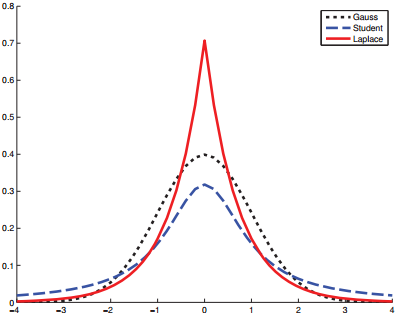
\includegraphics[scale=.70]{pdfs-for-NTL-a.png}} \\
\subfloat[]{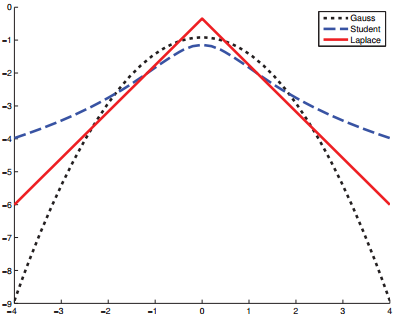
\includegraphics[scale=.70]{pdfs-for-NTL-b.png}}
\caption{(a) The pdf’s for a $\mathcal{N}(0,1)$, $\mathcal{T}(0,1,1)$ and $Lap(0,1/\sqrt{2})$. The mean is 0 and the variance is 1 for both the Gaussian and Laplace. The mean and variance of the Student is undefined when $\nu=1$.(b) Log of these pdf’s. Note that the Student distribution is not log-concave for any parameter value, unlike the Laplace distribution, which is always log-concave (and log-convex...) Nevertheless, both are unimodal.}
\label{fig:pdfs-for-NTL} 
\end{figure}

The variance is only defined if $\nu>2$. The mean is only defined if $\nu>1$.

As an illustration of the robustness of the Student distribution, consider Figure \ref{fig:robustness}. We see that the Gaussian is affected a lot, whereas the Student distribution hardly changes. This is because the Student has heavier tails, at least for small $\nu$(see Figure \ref{fig:pdfs-for-NTL}).

\begin{figure}[hbtp]
\centering
\subfloat[]{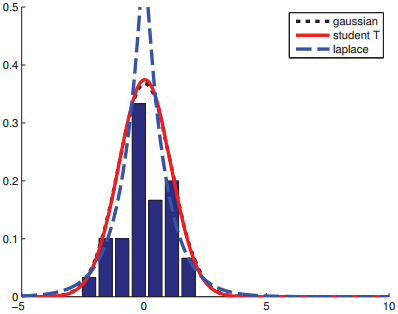
\includegraphics[scale=.70]{robustness-a.png}} \\
\subfloat[]{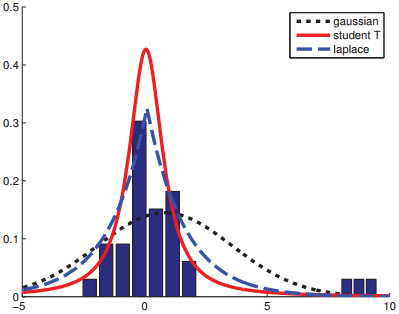
\includegraphics[scale=.70]{robustness-b.png}}
\caption{Illustration of the effect of outliers on fitting Gaussian, Student and Laplace distributions. (a) No outliers (the Gaussian and Student curves are on top of each other). (b) With outliers. We see that the Gaussian is more affected by outliers than the Student and Laplace distributions.}
\label{fig:robustness} 
\end{figure}

If $\nu=1$, this distribution is known as the \textbf{Cauchy} or \textbf{Lorentz} distribution. This is notable for having such heavy tails that the integral that defines the mean does not converge.

To ensure finite variance, we require $\nu>2$. It is common to use $\nu=4$, which gives good performance in a range of problems (Lange et al. 1989). For $\nu \gg 5$, the Student distribution rapidly approaches a Gaussian distribution and loses its robustness properties.


\subsection{The Laplace distribution}
\begin{table}
\caption{Summary of Laplace distribution.}
\centering
\begin{tabular}{cccccc}
\hline\noalign{\smallskip}
Written as & $f(x)$ & $\mathbb{E}[X]$ & mode & $\text{var}[X]$ \\
\noalign{\smallskip}\svhline\noalign{\smallskip}
$X \sim \text{Lap}(\mu,b)$ & $\dfrac{1}{2b}\exp\left(-\dfrac{|x-\mu|}{b}\right)$ & $\mu$ & $\mu$ & $2b^2$ \\
\noalign{\smallskip}\hline
\end{tabular}
\end{table}

Here $\mu$ is a location parameter and $b>0$ is a scale parameter. See Figure \ref{fig:pdfs-for-NTL} for a plot.

Its robustness to outliers is illustrated in Figure \ref{fig:robustness}. It also put mores probability density at 0 than the Gaussian. This property is a useful way to encourage sparsity in a model, as we will see in Section TODO.


\subsection{The gamma distribution}

\begin{table}
\caption{Summary of gamma distribution}
\centering
\begin{tabular}{ccccccc}
\hline\noalign{\smallskip}
Written as & $X$ & $f(x)$ & $\mathbb{E}[X]$ & mode & $\text{var}[X]$ \\
\noalign{\smallskip}\svhline\noalign{\smallskip}
$X \sim \text{Ga}(a,b)$ & $x \in \mathbb{R}^+$ & $\dfrac{b^a}{\Gamma(a)}x^{a-1}e^{-xb}$ & $\dfrac{a}{b}$ & $\dfrac{a-1}{b}$ & $\dfrac{a}{b^2}$ \\
\noalign{\smallskip}\hline
\end{tabular}
\end{table} 

Here $a>0$ is called the shape parameter and $b>0$ is called the rate parameter. See Figure \ref{fig:gamma-distribution} for some plots.

\begin{figure}[hbtp]
\centering
\subfloat[]{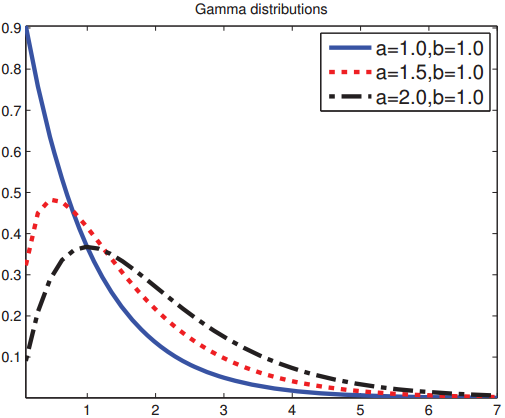
\includegraphics[scale=.50]{gamma-distribution-a.png}} \\
\subfloat[]{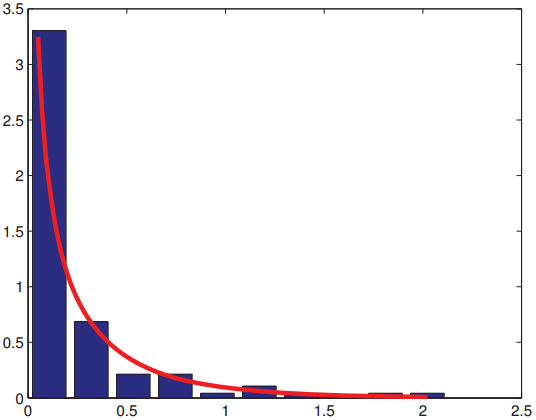
\includegraphics[scale=.50]{gamma-distribution-b.png}}
\caption{Some Ga$(a, b=1)$ distributions. If $a \leq 1$, the mode is at 0, otherwise it is $>0$.As we increase the rate $b$, we reduce the horizontal scale, thus squeezing everything leftwards and upwards. (b) An empirical pdf of some rainfall data, with a fitted Gamma distribution superimposed.}
\label{fig:gamma-distribution} 
\end{figure}


\subsection{The beta distribution}

\begin{table*}
\caption{Summary of Beta distribution}\label{tab:beta-distribution}
\centering
\begin{tabular}{ccccccc}
\hline\noalign{\smallskip}
Name & Written as & $X$ & $f(x)$ & $\mathbb{E}[X]$ & mode & $\text{var}[X]$ \\
\noalign{\smallskip}\svhline\noalign{\smallskip}
Beta distribution & $X \sim \text{Beta}(a,b)$ & $x \in [0,1]$ & $\dfrac{1}{B(a,b)}x^{a-1}(1-x)^{b-1}$ & $\dfrac{a}{a+b}$ & $\dfrac{a-1}{a+b-2}$ & $\dfrac{ab}{(a+b)^2(a+b+1)}$ \\
\noalign{\smallskip}\hline
\end{tabular}
\end{table*} 

Here $B(a, b)$is the beta function,
\begin{equation}
B(a,b) \triangleq \dfrac{\Gamma(a)\Gamma(b)}{\Gamma(a+b)}
\end{equation}

See Figure \ref{fig:beta-distribution} for plots of some beta distributions. We require  $a, b >0$ to ensure the distribution is integrable (i.e., to ensure $B(a, b)$ exists). If $a=b=1$, we get the uniform distirbution. If $a$ and $b$ are both less than 1, we get a bimodal distribution with “spikes” at 0 and 1; if $a$ and $b$ are both greater than 1, the distribution is unimodal.

\begin{figure}[hbtp]
\centering
    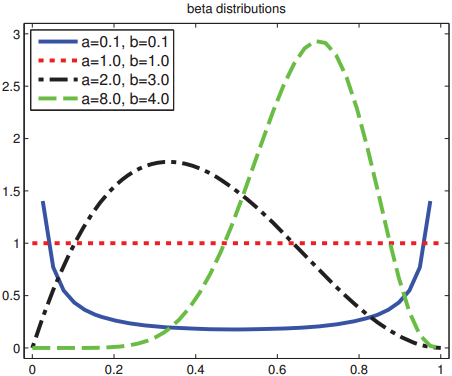
\includegraphics[scale=.60]{beta-distribution.png}
\caption{Some beta distributions.}
\label{fig:beta-distribution} 
\end{figure}


\subsection{Pareto distribution}

\begin{table*}
\caption{Summary of Pareto distribution}
\centering
\begin{tabular}{ccccccc}
\hline\noalign{\smallskip}
Name & Written as & $X$ & $f(x)$ & $\mathbb{E}[X]$ & mode & $\text{var}[X]$ \\
\noalign{\smallskip}\svhline\noalign{\smallskip}
Pareto distribution & $X \sim \text{Pareto}(k,m)$ & $x \geq m$ & $km^kx^{-(k+1)}\mathbb{I}(x \geq m)$ & $\dfrac{km}{k-1} \text{ if } k > 1$ & $m$ & $\dfrac{m^2k}{(k-1)^2(k-2)} \text{ if } k>2$ \\
\noalign{\smallskip}\hline
\end{tabular}
\end{table*} 

The \textbf{Pareto distribution} is used to model the distribution of quantities that exhibit \textbf{long tails}, also called \textbf{heavy tails}.

As $k \rightarrow \infty$, the distribution approaches $\delta(x-m)$. See Figure \ref{fig:Pareto-distribution}(a) for some plots. If we plot the distribution on a log-log scale, it forms a straight line, of the form $\log p(x)=a\log x+c$ for some constants $a$ and $c$. See Figure \ref{fig:Pareto-distribution}(b) for an illustration (this is known as a \textbf{power law}).

\begin{figure}[hbtp]
\centering
\subfloat[]{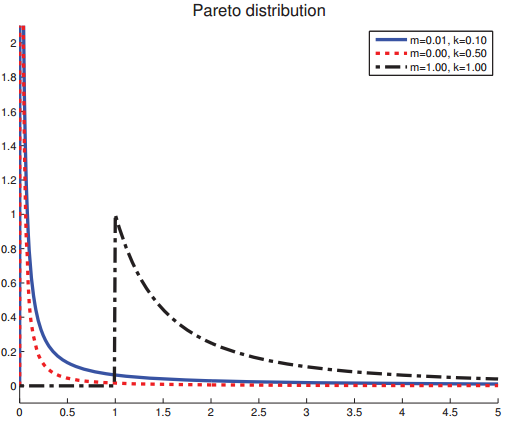
\includegraphics[scale=.50]{pareto-distribution-a.png}} \\
\subfloat[]{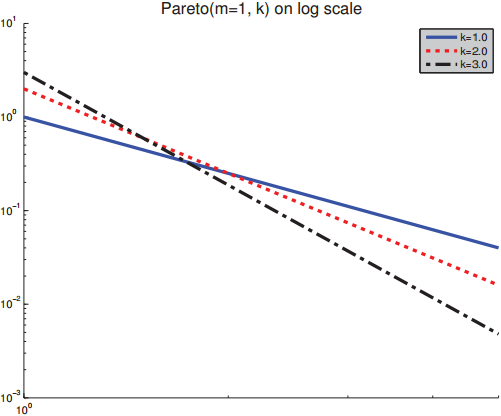
\includegraphics[scale=.50]{pareto-distribution-b.png}}
\caption{(a) The Pareto distribution Pareto$(x|m, k)$ for $m=1$. (b) The pdf on a log-log scale.}
\label{fig:Pareto-distribution} 
\end{figure}

\section{The Gaussian Distribution}
\label{sec:Gaussian distribution}
The Gaussian distributions,also known as the normal distributions,is a widely used model for the distribution of continuous variables.In the case of single variable $x$,the Gaussian is in the form
\begin{align}\label{eqn:univariate Gaussian distributions}
\mathcal{N}(x|\mu,\sigma^2)=\dfrac{1}{(2\pi\sigma^2)^{1/2}}\exp\{-\dfrac{1}{(2\sigma)^2}(x-\mu)^2 \}
\end{align}
where $\mu$ is the mean and $\sigma^2$ is the variance.For a $D$-dimensional vector $\vec{x}$,the multivariate Gaussian distribution takes the form
\begin{align}\label{eqn:multivariate Gaussian}
	\mathcal{N}(\vec{x}|\vec{\mu},\vec{\Sigma})
	=\dfrac{1}{(2\pi)^{D/2}}\dfrac{1}{\mid \vec{\Sigma}\mid^{1/2}}
	\exp\{-\dfrac{1}{2}(\vec{x}-\vec{\mu})^T\vec{\Sigma}^{-1}(\vec{x}-\vec{\mu}) \}
\end{align}
where $\vec{\mu}$ is a $D$-dimensional mean vector,$\vec{\Sigma}$ is a $D\times D$ covariance matrix,and $\mid\vec{\Sigma}\mid$ denotes the determinant of $\vec{\Sigma}$.

The Gaussian distribution arises in many different contexts and can be motivated from a variety of different perspectives,such as maximizing the entropy and the sum of multiple random variables.The \textbf{central limit theorem} tells us the latter.


\subsection{Conditional Gaussian distributions}
\subsection{Marginal Gaussian distributions}
\subsection{Baye's theorem for Gaussian variables}

\section{The exponential family}
\label{sec:exponential-family}

Before defining the exponential family, we mention several reasons why it is important:
\begin{itemize}
	\item{It can be shown that, under certain regularity conditions, the exponential family is the only family of distributions with finite-sized sufficient statistics, meaning that we can compress the data into a fixed-sized summary without loss of information. This is particularly useful for online learning, as we will see later.}
	\item{The exponential family is the only family of distributions for which conjugate priors exist, which simplifies the computation of the posterior (see Section \ref{sec:Bayes-for-the-exponential-family}).}
	\item{The exponential family can be shown to be the family of distributions that makes the least set of assumptions subject to some user-chosen constraints (see Section \ref{sec:Maximum-entropy-derivation-of-the-exponential-family}).}
	\item{The exponential family is at the core of generalized linear models, as discussed in Section \ref{sec:GLMs}.}
	\item{The exponential family is at the core of variational inference, as discussed in Section TODO.}
\end{itemize}


\subsection{Definition}
A pdf or pmf $p(\vec{x}|\vec{\theta})$,for $\vec{x} \in \mathbb{R}^m$ and $\vec{\theta} \in \mathbb{R}^D$, is said to be in the \textbf{exponential family} if it is of the form
\begin{align}
p(\vec{x}|\vec{\theta}) 
&= h(\vec{x})g(\vec{\theta})\exp\{\vec{\theta}^T\vec{\phi}(\vec{x})\} \\
&=\dfrac{1}{Z(\vec{\theta})}h(\vec{x})\exp[\vec{\theta}^T\phi(\vec{x})] \\
& = h(\vec{x})\exp[\vec{\theta}^T\phi(\vec{x})-A(\vec{\theta})] \label{eqn:exponential-family}
\end{align}
where
\begin{align}
Z(\vec{\theta}) & =\int h(\vec{x})\exp[\vec{\theta}^T\phi(\vec{x})]\mathrm{d}\vec{x} \\
A(\vec{\theta}) & =\log Z(\vec{\theta})
\end{align}

Here $\vec{\theta}$ are called the \textbf{natural parameters} or \textbf{canonical parameters}, $\phi(\vec{x}) \in \mathbb{R}^D$ is called a vector of \textbf{sufficient statistics}, $Z(\vec{\theta})$ is called the \textbf{partition function}, $A(\vec{\theta})$ is called the \textbf{log partition function} or \textbf{cumulant function}, and $h(\vec{x})$ is the a scaling constant, often 1. If $\phi(\vec{x})=\vec{x}$, we say it is a \textbf{natural exponential family}.

Equation \ref{eqn:exponential-family} can be generalized by writing
\begin{equation}
p(\vec{x}|\vec{\theta}) = h(\vec{x})\exp[\eta(\vec{\theta})^T\phi(\vec{x})-A(\eta(\vec{\theta}))]
\end{equation}
where $\eta$ is a function that maps the parameters $\vec{\theta}$ to the canonical parameters $\vec{\eta}=\eta(\vec{\theta})$.If $\mathrm{dim}(\vec{\theta})<\mathrm{dim}(\eta(\vec{\theta}))$, it is called a \textbf{curved exponential family}, which means we have more sufficient statistics than parameters. If $\eta(\vec{\theta})=\vec{\theta}$, the model is said to be in \textbf{canonical form}. We will assume models are in canonical form unless we state otherwise.

\subsection{Maximum likelihood and sufficient statistics}

\subsection{Conjugate priors}

\subsection{Noninformative prios}
In many cases,however,we may have little idea of what form the distribution should take.We may then seek a form of prior distribution,called a \textbf{noninformative prior},which is intended to have little influence on the posterior distribution as possible(Jeffries,1946;Box and Tao,1973;Bernardo and Smith,1994).

Suppose we have a distribution $p(x|\lambda)$ governed by a parameter $\lambda$,we might be tempted to propose a prior distribution $p(\lambda) = $const as a suitable prior.Improper priors are ones in which the domain $\lambda$ is unbounded and the prior distribution cannot be correctly normalized because the integral over $\lambda$ diverges.A second difficulty arises from the transformation behaviour of a probability density under a nonlinear change of variables.For example
\begin{equation}
p_\eta(\eta) = p_\lambda(\lambda) \left | \dfrac{d\lambda}{d\eta} \right | = p_\lambda(\eta^2)\eta\propto \eta
\end{equation}
so the density over $\eta$ will not be constant.

Here are two simple examples of noninformative priors(Berger,1985).
First of all,if a density takes the form
\begin{equation}
p(x|\mu) = f(x-\mu)
\end{equation}
then the parameter $\mu$ is known as a \textbf{location parameter}.This family of densities exhibits \textbf{translation invariance} because if we shift $x$ by a constant to give $\hat{x} = x+c$,then
\begin{equation}
p(\hat{x}|\hat{\mu}) = f(\hat{x}-\hat{\mu})
\end{equation}
where $\hat{\mu} = \mu +c$.

A second example,
\begin{equation}\label{eqn:density scale parameter}
p(x|\sigma) = \dfrac{1}{\sigma}f(\dfrac{x}{\sigma})
\end{equation}
where $\sigma>0$.Note that this will be a normalized density provided f(x) is correctly normalized.The parameter $\sigma$ is known as a \textbf{scale parameter},and the density exhibits \textbf{scale invariance}.

\subsection{Examples}


\subsubsection{Bernoulli}
The Bernoulli for $x \in \{0,1\}$ can be written in exponential family form as follows:
\begin{equation}\begin{split}
\mathrm{Ber}(x|\mu)& =\mu^x(1-\mu)^{1-x} \\
& =\exp[x\log\mu+(1-x)\log(1-\mu)]
\end{split}\end{equation}
where $\phi(x)=(\mathbb{I}(x=0),\mathbb{I}(x=1))$ and $\vec{\theta}=(\log\mu,\log(1-\mu))$. 

However, this representation is \textbf{over-complete} since $\vec{1}^T\phi(x)=\mathbb{I}(x=0)+\mathbb{I}(x=1)=1$. Consequently $\vec{\theta}$ is not uniquely identifiable. It is common to require that the representation be \textbf{minimal}, which means there is a unique $\theta$ associated with the distribution. In this case, we can just define
\begin{align}
\mathrm{Ber}(x|\mu) & =(1-\mu)\exp\left(x\log\dfrac{\mu}{1-\mu}\right) \\
\text{where } \phi(x) & =x, \theta=\log\dfrac{\mu}{1-\mu}, Z=\dfrac{1}{1-\mu}  \nonumber
\end{align}

We can recover the mean parameter $\mu$ from the canonical parameter using
\begin{equation}
\mu=\mathrm{sigm}(\theta)=\dfrac{1}{1+e^{-\theta}}
\end{equation}


\subsubsection{Multinoulli}
We can represent the multinoulli as a minimal exponential family as follows:
\begin{equation*}\begin{split}
& \mathrm{Cat}(\vec{x}|\vec{\mu}) = \prod\limits_{k=1}^K = \exp\left(\sum\limits_{k=1}^K x_k\log\mu_k\right) \\
& = \exp\left[\sum\limits_{k=1}^{K-1} x_k\log\mu_k+  (1-\sum\limits_{k=1}^{K-1} x_k)\log(1-\sum\limits_{k=1}^{K-1} \mu_k)\right] \\
& = \exp\left[\sum\limits_{k=1}^{K-1} x_k\log\dfrac{\mu_k}{1-\sum_{k=1}^{K-1} \mu_k} + \log(1-\sum\limits_{k=1}^{K-1} \mu_k) \right] \\
& = \exp\left[\sum\limits_{k=1}^{K-1} x_k\log\dfrac{\mu_k}{\mu_K}+\log\mu_K\right] \text{, where } \mu_K \triangleq 1-\sum\limits_{k=1}^{K-1} \mu_k
\end{split}\end{equation*}

We can write this in exponential family form as follows:
\begin{align}
\mathrm{Cat}(\vec{x}|\vec{\mu}) & = \exp[\vec{\theta}^T\phi(\vec{x})-A(\vec{\theta})] \\
\vec{\theta} & \triangleq (\log\dfrac{\mu_1}{\mu_K},\cdots,\log\dfrac{\mu_{K-1}}{\mu_K}) \\
\phi(\vec{x}) & \triangleq (x_1,\cdots,x_{K-1})
\end{align}

We can recover the mean parameters from the canonical parameters using
\begin{align}
\mu_k & = \dfrac{e^{\theta_k}}{1+\sum_{j=1}^{K-1} e^{\theta_j}} \\
\mu_K & = 1- \dfrac{\sum_{j=1}^{K-1} e^{\theta_j}}{1+\sum_{j=1}^{K-1} e^{\theta_j}}=\dfrac{1}{1+\sum_{j=1}^{K-1} e^{\theta_j}}
\end{align}
and hence
\begin{equation}
A(\vec{\theta]} = -\log\mu_K=\log(1+\sum\limits_{j=1}^{K-1} e^{\theta_j})
\end{equation}


\subsubsection{Univariate Gaussian}
The univariate Gaussian can be written in exponential family form as follows:
\begin{align}
\mathcal{N}(x|\mu,\sigma^2) & =\dfrac{1}{\sqrt{2\pi}\sigma}\exp\left[-\dfrac{1}{2\sigma^2}(x-\mu)^2\right] \nonumber \\
& = \dfrac{1}{\sqrt{2\pi}\sigma}\exp\left[-\dfrac{1}{2\sigma^2}x^2+\dfrac{\mu}{\sigma^2}x-\dfrac{1}{2\sigma^2}\mu^2\right] \nonumber \\
& = \dfrac{1}{Z(\vec{\theta})}\exp[\vec{\theta}^T\phi(x)]
\end{align}
where
\begin{align}
\vec{\theta} & = (\dfrac{\mu}{\sigma^2}, -\dfrac{1}{2\sigma^2}) \\
\phi(x) & =(x,x^2) \\
Z(\vec{\theta}) & =\sqrt{2\pi}\sigma\exp(\dfrac{\mu^2}{2\sigma^2})
\end{align}


\subsubsection{Non-examples}
Not all distributions of interest belong to the exponential family. For example, the uniform distribution,$X \sim U(a,b)$, does not, since the support of the distribution depends on the parameters. Also, the Student T distribution (Section TODO) does not belong, since it does not have the required form.


\subsection{Log partition function}
An important property of the exponential family is that derivatives of the log partition function can be used to generate \textbf{cumulants} of the sufficient statistics.\footnote{The first and second cumulants of a distribution are its mean $\mathbb{E}[X]$ and variance $\mathrm{var}[X]$, whereas the first and second moments are its mean $\mathbb{E}[X]$ and $\mathbb{E}[X^2]$.} For this reason, $A(\vec{\theta})$ is sometimes called a \textbf{cumulant function}. We will prove this for a 1-parameter distribution; this can be generalized to a $K$-parameter distribution in a straightforward way. For the first derivative we have

For the second derivative we have
\begin{align}
\dfrac{\mathrm{d} A}{\mathrm{d} \theta} & = \dfrac{\mathrm{d}}{\mathrm{d} \theta}\left\{\log\int\exp\left[\theta\phi(x)\right]h(x)\mathrm{d}x\right\} \nonumber \\
& = \dfrac{\frac{\mathrm{d}}{\mathrm{d} \theta}\int\exp\left[\theta\phi(x)\right]h(x)\mathrm{d}x}{\int\exp\left[\theta\phi(x)\right]h(x)\mathrm{d}x} \nonumber \\
& = \dfrac{\int\phi(x)exp\left[\theta\phi(x)\right]h(x)\mathrm{d}x}{\exp(A(\theta))} \nonumber \\
& = \int \phi(x)\exp\left[\theta\phi(x)-A(\theta)\right]h(x)\mathrm{d}x \nonumber \\
& = \int \phi(x)p(x)\mathrm{d}x=\mathbb{E}[\phi(x)]
\end{align}

For the second derivative we have
\begin{align}
\dfrac{\mathrm{d}^2 A}{\mathrm{d} \theta^2} & = \int \phi(x)\exp\left[\theta\phi(x)-A(\theta)\right]h(x)\left[\phi(x)-A'(\theta)\right]\mathrm{d}x \nonumber \\
& = \int \phi(x)p(x)\left[\phi(x)-A'(\theta)\right]\mathrm{d}x \nonumber \\
& = \int \phi^2(x)p(x)\mathrm{d}x-A'(\theta)\int \phi(x)p(x)\mathrm{d}x \nonumber \\
& = \mathbb{E}[\phi^2(x)]-\mathbb{E}[\phi(x)]^2=\mathrm{var}[\phi(x)]
\end{align}

In the multivariate case, we have that
\begin{equation}
\dfrac{\partial^2 A}{\partial \theta_i \partial \theta_j}=\mathbb{E}[\phi_i(x)\phi_j(x)]-\mathbb{E}[\phi_i(x)]\mathbb{E}[\phi_j(x)]
\end{equation}
and hence
\begin{equation}
\nabla^2A(\vec{\theta}) = \mathrm{cov}[\phi(\vec{x})]
\end{equation}

Since the covariance is positive definite, we see that $A(\vec{\theta})$ is a convex function (see Section \ref{sec:Convexity}).


\subsection{MLE for the exponential family}
The likelihood of an exponential family model has the form
\begin{equation}
p(\mathcal{D}|\vec{\theta})=\left[\prod\limits_{i=1}^N h(\vec{x}_i)\right]g(\vec{\theta})^N\exp\left[\vec{\theta}^T\left(\sum\limits_{i=1}^N \phi(\vec{x}_i)\right)\right]
\end{equation}

We see that the sufficient statistics are $N$ and
\begin{equation}
\phi(\mathcal{D})=\sum\limits_{i=1}^N \phi(\vec{x}_i)=(\sum\limits_{i=1}^N \phi_1(\vec{x}_i),\cdots,\sum\limits_{i=1}^N \phi_K(\vec{x}_i))
\end{equation}

The \textbf{Pitman-Koopman-Darmois theorem} states that, under certain regularity conditions, the exponential family is the only family of distributions with finite sufficient statistics. (Here, finite means of a size independent of the size of the data set.)

One of the conditions required in this theorem is that the support of the distribution not be dependent on the parameter.


\subsection{Bayes for the exponential family}
\label{sec:Bayes-for-the-exponential-family}
TODO


\subsubsection{Likelihood}



\subsection{Maximum entropy derivation of the exponential family *}
\label{sec:Maximum-entropy-derivation-of-the-exponential-family}


\section{Nonparametric Methods}
\subsection{Kernel density estimators}
\subsection{Nearest-neighbour methods}


\section{Joint probability distributions}
Given a \textbf{multivariate random variable} or \textbf{random vector} \footnote{\url{http://en.wikipedia.org/wiki/Multivariate_random_variable}} $X \in \mathbb{R}^D$, the \textbf{joint probability distribution}\footnote{\url{http://en.wikipedia.org/wiki/Joint_probability_distribution}} is a probability distribution that gives the probability that each of $X_1, X_2, \cdots,X_D$ falls in any particular range or discrete set of values specified for that variable. In the case of only two random variables, this is called a \textbf{bivariate distribution}, but the concept generalizes to any number of random variables, giving a \textbf{multivariate distribution}.

The joint probability distribution can be expressed either in terms of a \textbf{joint cumulative distribution function} or in terms of a \textbf{joint probability density function} (in the case of continuous variables) or \textbf{joint probability mass function} (in the case of discrete variables). 


\subsection{Covariance and correlation}
\begin{definition}
The \textbf{covariance} between two rv’s $X$ and $Y$ measures the degree to which $X$ and $Y$ are (linearly) related. Covariance is defined as
\begin{equation}
\begin{split}
\mathrm{cov}[X,Y] & \triangleq \mathbb{E}\left[(X-\mathbb{E}[X])(Y-\mathbb{E}[Y])\right] \\
         & =\mathbb{E}[XY]-\mathbb{E}[X]\mathbb{E}[Y]
\end{split}
\end{equation}
\end{definition}

\begin{definition}
If $X$ is a $D$-dimensional random vector, its \textbf{covariance matrix} is defined to be the following symmetric, positive definite matrix:
\begin{align}
\mathrm{cov}[\vec{x}] & \triangleq \mathbb{E}\left[(\vec{x}-\mathbb{E}[\vec{x}])(\vec{x}-\mathbb{E}[\vec{x}])^T\right] \\
       &  = \left( \begin{array}{cccc}
           \text{var}[\vec{x_1}] & \text{Cov}[\vec{x_1},\vec{x_2}] & \cdots & \text{Cov}[\vec{x_1},\vec{x_D}] \\
           \text{Cov}[\vec{x_2},\vec{x_1}] & \text{var}[x_2] & \cdots & \text{Cov}[\vec{x_2},\vec{x_D}] \\
		   \vdots & \vdots & \ddots & \vdots \\
           \text{Cov}[\vec{x_D},\vec{x_1}] & \text{Cov}[\vec{x_D},\vec{x_2}] & \cdots & \text{var}[\vec{x_D}] \end{array} \right)
\end{align}
\end{definition}
For 

\begin{definition}
The (Pearson) \textbf{correlation coefficient} between $X$ and $Y$ is defined as
\begin{equation}
\text{corr}[X,Y] \triangleq \dfrac{\text{Cov}[X,Y]}{\sqrt{\text{var}[X],\text{var}[Y]}}
\end{equation}
\end{definition}

A \textbf{correlation matrix} has the form
\begin{equation}
\mathbf{R} \triangleq \left( \begin{array}{cccc}
           \text{corr}[X_1,X_1] & \text{corr}[X_1,X_2] & \cdots & \text{corr}[X_1,X_D] \\
           \text{corr}[X_2,X_1] & \text{corr}[X_2,X_2] & \cdots & \text{corr}[X_2,X_D] \\
		   \vdots & \vdots & \ddots & \vdots \\
           \text{corr}[X_D,X_1] & \text{corr}[X_D,X_2] & \cdots & \text{corr}[X_D,X_D] \end{array} \right)
\end{equation}

The correlation coefficient can viewed as a degree of linearity between $X$ and $Y$, see Figure \ref{fig:Correlation-examples}.
\begin{figure*}[hbtp]
\centering
    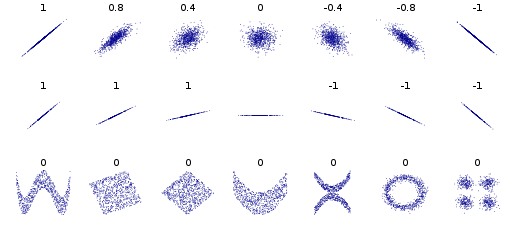
\includegraphics[scale=.80]{Correlation-examples.png}
\caption{Several sets of $(x, y)$ points, with the Pearson correlation coefficient of $x$ and $y$ for each set. Note that the correlation reflects the noisiness and direction of a linear relationship (top row), but not the slope of that relationship (middle), nor many aspects of nonlinear relationships (bottom). N.B.: the figure in the center has a slope of 0 but in that case the correlation coefficient is undefined because the variance of $Y$ is zero.Source:\url{http://en.wikipedia.org/wiki/Correlation}}
\label{fig:Correlation-examples} 
\end{figure*}

\textbf{Uncorrelated does not imply independent}. For example, let $X \sim U(-1,1)$ and $Y =X^2$. Clearly $Y$ is dependent on $X$(in fact, $Y$ is uniquely determined by $X$), yet one can show that corr$[X, Y]=0$. Some striking examples of this fact are shown in Figure \ref{fig:Correlation-examples}. This shows several data sets where there is clear dependence between $X$ and $Y$, and yet the correlation coefficient is 0. A more general measure of dependence between random variables is mutual information, see Section TODO.


\subsection{Multivariate Gaussian distribution}
\label{sec:MVN}
The \textbf{multivariate Gaussian} or \textbf{multivariate normal}(MVN) is the most widely used joint probability density function for continuous variables. We discuss MVNs in detail in Chapter 4; here we just give some definitions and plots.

The pdf of the MVN in $D$ dimensions is defined by the following:
\begin{equation}
\mathcal{N}(\vec{x}|\vec{\mu},\Sigma) \triangleq \dfrac{1}{(2\pi)^{D/2}|\Sigma|^{1/2}}\exp\left[-\dfrac{1}{2}(\vec{x}-\vec{\mu})^T\Sigma^{-1}(\vec{x}-\vec{\mu})\right]
\end{equation}
where $\vec{\mu}=\mathbb{E}[X] \in \mathbb{R}^D$ is the mean vector, and $\Sigma=\text{Cov}[X]$ is the $D \times D$ covariance matrix. The normalization constant $(2\pi)^{D/2}|\Sigma|^{1/2}$ just ensures that the pdf integrates to 1.

Figure \ref{fig:2d-Gaussions} plots some MVN densities in 2d for three different kinds of covariance matrices. A full covariance matrix has A $D(D+1)/2$ parameters (we divide by 2 since $\Sigma$ is symmetric). A diagonal covariance matrix has $D$ parameters, and has 0s in the off-diagonal terms. A spherical or isotropic covariance,$\Sigma=\sigma^2\vec{I}_D$, has one free parameter.

\begin{figure}[hbtp]
\centering
\subfloat[]{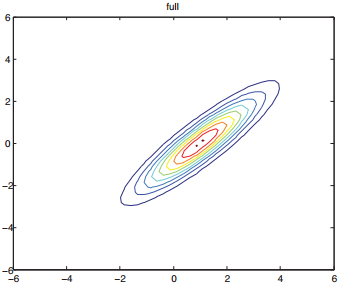
\includegraphics[scale=.60]{2d-Gaussions-a.png}} \\
\subfloat[]{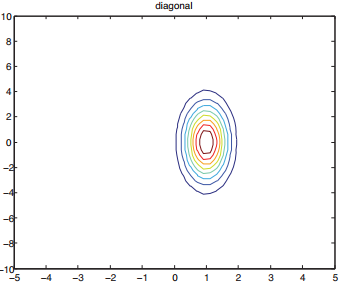
\includegraphics[scale=.60]{2d-Gaussions-b.png}} \\
\subfloat[]{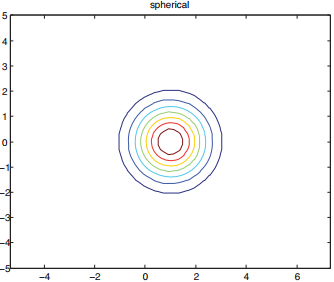
\includegraphics[scale=.60]{2d-Gaussions-c.png}} \\
\subfloat[]{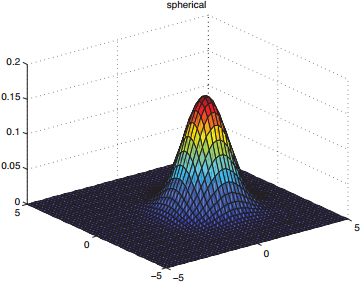
\includegraphics[scale=.60]{2d-Gaussions-d.png}}
\caption{We show the level sets for 2d Gaussians. (a) A full covariance matrix has elliptical contours.(b) A diagonal covariance matrix is an axis aligned ellipse. (c) A spherical covariance matrix has a circular shape. (d) Surface plot for the spherical Gaussian in (c).}
\label{fig:2d-Gaussions} 
\end{figure}


\subsection{Multivariate Student's t-distribution}
A more robust alternative to the MVN is the multivariate Student's t-distribution, whose pdf is given by
\begin{align}
& \mathcal{T}(x|\vec{\mu},\Sigma,\nu) \nonumber \\
& \triangleq \dfrac{\Gamma(\frac{\nu+D}{2})}{\Gamma(\frac{\nu}{2})}\dfrac{|\Sigma|^{-\frac{1}{2}}}{\left(\nu\pi\right)^{\frac{D}{2}}}\left[1+\dfrac{1}{\nu}\left(\vec{x}-\vec{\mu}\right)^T\Sigma^{-1}\left(\vec{x}-\vec{\mu}\right)\right]^{-\frac{\nu+D}{2}} \\
&= \dfrac{\Gamma(\frac{\nu+D}{2})}{\Gamma(\frac{\nu}{2})}\dfrac{|\Sigma|^{-\frac{1}{2}}}{\left(\nu\pi\right)^{\frac{D}{2}}}\left[1+\left(\vec{x}-\vec{\mu}\right)^T\vec{V}^{-1}\left(\vec{x}-\vec{\mu}\right)\right]^{-\frac{\nu+D}{2}}
\end{align}
where $\Sigma$ is called the scale matrix (since it is not exactly the covariance matrix) and $\vec{V}=\nu\Sigma$. This has fatter tails than a Gaussian. The smaller $\nu$ is, the fatter the tails. As $\nu \rightarrow \infty$, the distribution tends towards a Gaussian. The distribution has the following properties
\begin{equation}
\text{mean}=\vec{\mu} \text{ , mode}=\vec{\mu} \text{ , Cov}= \dfrac{\nu}{\nu-2}\Sigma
\end{equation}


\subsection{Dirichlet distribution}
A multivariate generalization of the beta distribution is the \textbf{Dirichlet distribution}, which has
support over the probability simplex, defined by
\begin{equation}
S_K=\left\{\vec{x}:0 \leq x_k \leq 1,\sum\limits_{k=1}^K x_k=1\right\}
\end{equation}

The pdf is defined as follows:
\begin{equation}
\text{Dir}(\vec{x}|\vec{\alpha}) \triangleq \dfrac{1}{B(\vec{\alpha})}\prod\limits_{k=1}^K x_k^{\alpha_k-1}\mathbb{I}(\vec{x} \in S_K)
\end{equation}
where $B(\alpha_1,\alpha_2,\cdots,\alpha_K)$ is the natural generalization of the beta function to $K$ variables:
\begin{equation}
B(\alpha) \triangleq \dfrac{\prod_{k=1}^K \Gamma(\alpha_k)}{\Gamma(\alpha_0)} \text{ where } \alpha_0 \triangleq \sum_{k=1}^K \alpha_k
\end{equation}

Figure \ref{fig:3d-Dirichlet} shows some plots of the Dirichlet when $K=3$, and Figure \ref{fig:5d-Dirichlet} for some sampled probability vectors. We see that $\alpha_0$ controls the strength of the distribution (how peaked it is), and theαkcontrol where the peak occurs. For example, Dir$(1,1,1)$ is a uniform distribution, Dir$(2,2,2)$ is a broad distribution centered at $(1/3,1/3,1/3)$, and Dir$(20,20,20)$ is a narrow distribution centered at $(1/3,1/3,1/3)$.If $\alpha_k < 1$ for all $k$, we get “spikes” at the corner of the simplex.

\begin{figure}[hbtp]
\centering
\subfloat[]{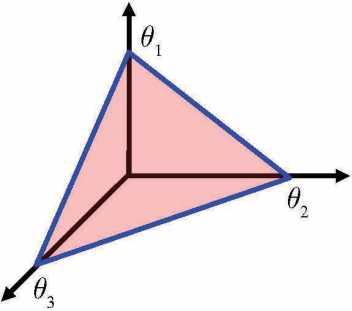
\includegraphics[scale=.50]{3d-Dirichlet-a.png}} \\
\subfloat[]{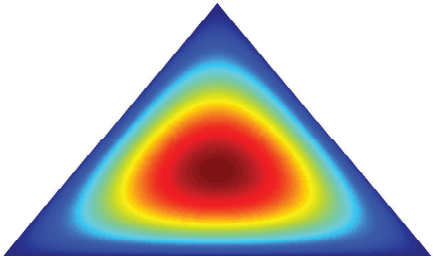
\includegraphics[scale=.60]{3d-Dirichlet-b.png}} \\
\subfloat[]{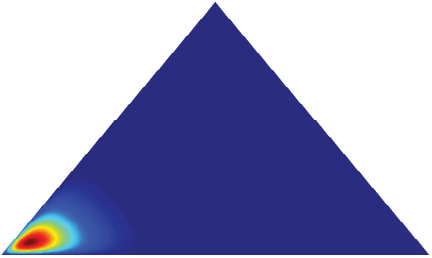
\includegraphics[scale=.60]{3d-Dirichlet-c.png}} \\
\subfloat[]{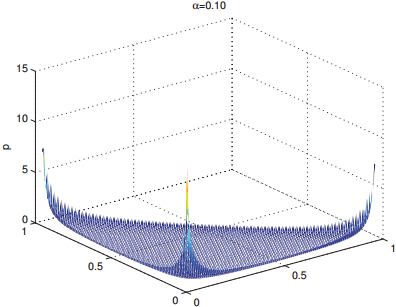
\includegraphics[scale=.60]{3d-Dirichlet-d.png}}
\caption{(a) The Dirichlet distribution when $K=3$ defines a distribution over the simplex, which can be represented by the triangular surface. Points on this surface satisfy $0 \leq \theta_k \leq 1$ and $\sum_{k=1}^K \theta_k=1$. (b) Plot of the Dirichlet density when $\vec{\alpha}=(2,2,2)$. (c) $\vec{\alpha}=(20,2,2)$.}
\label{fig:3d-Dirichlet} 
\end{figure}

\begin{figure}[hbtp]
\centering
\subfloat[$\vec{\alpha}=(0.1,\cdots,0.1)$. This results in very sparse distributions, with many 0s.]{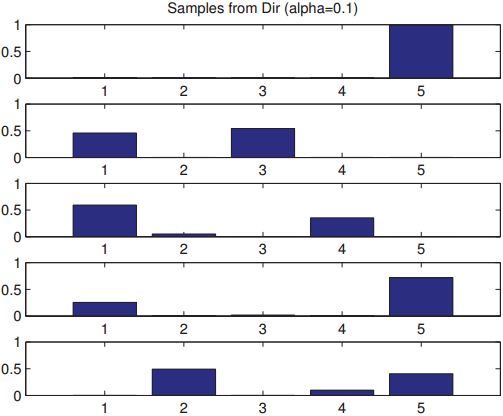
\includegraphics[scale=.50]{5d-Dirichlet-a.png}} \\
\subfloat[$\vec{\alpha}=(1,\cdots,1)$. This results in more uniform (and dense) distributions.]{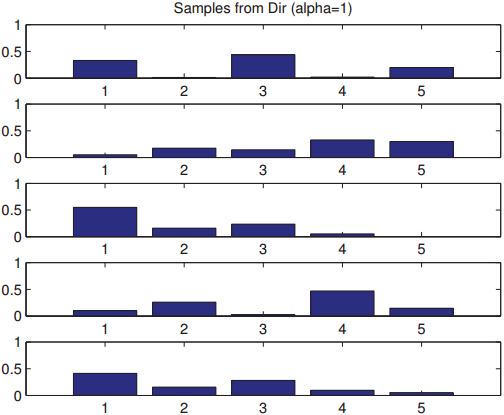
\includegraphics[scale=.50]{5d-Dirichlet-b.png}}
\caption{Samples from a 5-dimensional symmetric Dirichlet distribution for different parameter values.} 
\label{fig:5d-Dirichlet} 
\end{figure}

For future reference, the distribution has these properties
\begin{equation}\label{eqn:Dirichlet-properties}
\mathbb{E}(x_k)=\dfrac{\alpha_k}{\alpha_0} \text{, mode}[x_k]=\dfrac{\alpha_k-1}{\alpha_0-K} \text{, var}[x_k]=\dfrac{\alpha_k(\alpha_0-\alpha_k)}{\alpha_0^2(\alpha_0+1)}
\end{equation}


\section{Transformations of random variables}
If $\vec{x} \sim P()$ is some random variable, and $\vec{y}=f(\vec{x})$, what is the distribution of $Y$? This is the question we address in this section.


\subsection{Linear transformations}
Suppose $g()$ is a linear function: 
\begin{equation}
g(\vec{x})=A\vec{x}+b
\end{equation}

First, for the mean, we have
\begin{equation}
\mathbb{E}[\vec{y}]=\mathbb{E}[A\vec{x}+b]=A\mathbb{E}[\vec{x}]+b
\end{equation}
this is called the \textbf{linearity of expectation}.

For the covariance, we have
\begin{equation}
\text{Cov}[\vec{y}]=\text{Cov}[A\vec{x}+b]=A\Sigma A^T
\end{equation}


\subsection{General transformations}
\label{sec:General-transformations}
If $X$ is a discrete rv, we can derive the pmf for $y$ by simply summing up the probability mass for all the $x$’s such that $f(x)=y$:
\begin{equation}\label{eqn:transformation-discrete}
p_Y(y)=\sum\limits_{x:g(x)=y}p_X(x)
\end{equation}

If $X$ is continuous, we cannot use Equation \ref{eqn:transformation-discrete} since $p_X(x)$ is a density, not a pmf, and we cannot sum up densities. Instead, we work with cdf’s, and write
\begin{equation}
F_Y(y)=P(Y \leq y)=P(g(X) \leq y)=\int\limits_{g(X) \leq y} f_X(x)\mathrm{d}x
\end{equation}

We can derive the pdf of $Y$ by differentiating the cdf:
\begin{equation}\label{eqn:General-transformations}
f_Y(y)=f_X(x)|\dfrac{dx}{dy}|
\end{equation}

This is called \textbf{change of variables} formula. We leave the proof of this as an exercise. 

For example, suppose $X \sim U(−1,1)$, and $Y=X^2$. Then $p_Y(y)=\dfrac{1}{2}y^{-\frac{1}{2}}$.


\subsubsection{Multivariate change of variables *}
Let $f$ be a function $f:\mathbb{R}^n \rightarrow \mathbb{R}^n$, and let $\vec{y}=f(\vec{x})$. Then its Jacobian matrix $\vec{J}$ is given by
\begin{equation}
\vec{J}_{\vec{x} \rightarrow \vec{y}} \triangleq \frac{\partial \vec{y}}{\partial \vec{x}} \triangleq \left(\begin{array}{ccc}
\frac{\partial y_1}{\partial x_1} & \cdots & \frac{\partial y_1}{\partial x_n} \\
\vdots & \vdots & \vdots \\
\frac{\partial y_n}{\partial x_1} & \cdots & \frac{\partial y_n}{\partial x_n}
\end{array}\right)
\end{equation}
$|\mathrm{det}(\vec{J})|$ measures how much a unit cube changes in volume when we apply $f$.

If $f$ is an invertible mapping, we can define the pdf of the transformed variables using the Jacobian of the inverse mapping $\vec{y} \rightarrow \vec{x}$:
\begin{equation}\label{eqn:Multivariate-transformation}
p_y(\vec{y})=p_x(\vec{x})|\mathrm{det}(\frac{\partial \vec{x}}{\partial \vec{y}})|=p_x(\vec{x})|\mathrm{det}(\vec{J}_{\vec{y} \rightarrow \vec{x}})|
\end{equation}


\subsection{Central limit theorem}
Given $N$ random variables $X_1,X_2,\cdots,X_N$, each variable is \textbf{independent and identically distributed}\footnote{\url{http://en.wikipedia.org/wiki/Independent_identically_distributed}}(\textbf{iid} for short), and each has the same mean $\mu$ and variance $\sigma^2$, then
\begin{equation}
\dfrac{\sum\limits_{i=1}^n X_i-N\mu}{\sqrt{N}\sigma} \sim \mathcal{N}(0,1)
\end{equation}
this can also be written as
\begin{equation}
\dfrac{\bar{X}-\mu}{\sigma/\sqrt{N}} \sim \mathcal{N}(0,1) \quad \text{, where } \bar{X} \triangleq \dfrac{1}{N}\sum\limits_{i=1}^n X_i
\end{equation}


\section{Monte Carlo approximation}
\label{sec:Monte-Carlo-approximation}
In general, computing the distribution of a function of an rv using the change of variables formula can be difficult. One simple but powerful alternative is as follows. First we generate $S$ samples from the distribution, call them $x_1,\cdots,x_S$. (There are many ways to generate such samples; one popular method, for high dimensional distributions, is called Markov chain Monte Carlo or MCMC; this will be explained in Chapter TODO.) Given the samples, we can approximate the distribution of $f(X)$ by using the empirical distribution of $\left\{f(x_s)\right\}_{s=1}^S$. This is called a \textbf{Monte Carlo approximation}\footnote{\url{http://en.wikipedia.org/wiki/Monte_Carlo_method}}, named after a city in Europe known for its plush gambling casinos.

We can use Monte Carlo to approximate the expected value of any function of a random variable. We simply draw samples, and then compute the arithmetic mean of the function applied to the samples. This can be written as follows:
\begin{equation}
\mathbb{E}[g(X)]=\int g(x)p(x)\mathrm{d}x \approx \dfrac{1}{S}\sum\limits_{s=1}^S f(x_s)
\end{equation}
where $x_s \sim p(X)$.

This is called \textbf{Monte Carlo integration}\footnote{\url{http://en.wikipedia.org/wiki/Monte_Carlo_integration}}, and has the advantage over numerical integration (which is based on evaluating the function at a fixed grid of points) that the function is only evaluated in places where there is non-negligible probability.


\section{Information theory}

\subsection{Entropy}
\label{sec:Entropy}
The entropy of a random variable $X$ with distribution $p$, denoted by $\mathbb{H}(X)$ or sometimes $\mathbb{H}(p)$, is a measure of its uncertainty. In particular, for a discrete variable with $K$ states, it is defined by
\begin{equation}
\mathbb{H}(X) \triangleq -\sum\limits_{k=1}^{K}{p(X=k)\log_2p(X=k)}
\end{equation}

Usually we use log base 2, in which case the units are called \textbf{bits}(short for binary digits). If we use log base $e$ , the units are called \textbf{nats}. 

The discrete distribution with maximum entropy is the uniform distribution (see Section XXX for a proof). Hence for a K-ary random variable, the entropy is maximized if $p(x = k)=1/K$; in this case, $\mathbb{H}(X)=\log_2K$. 

Conversely, the distribution with minimum entropy (which is zero) is any \textbf{delta-function} that puts all its mass on one state. Such a distribution has no uncertainty.


\subsection{KL divergence}
One way to measure the dissimilarity of two probability distributions, $p$ and $q$ , is known as the \textbf{Kullback-Leibler divergence}(\textbf{KL divergence})or \textbf{relative entropy}. This is defined as follows:
\begin{equation}
\mathbb{KL}(P||Q) \triangleq 
\sum\limits_{x}{p(x)\log_2\dfrac{p(x)}{q(x)}}
\end{equation}
where the sum gets replaced by an integral for pdfs\footnote{The KL divergence is not a distance, since it is asymmetric. One symmetric version of the KL divergence is the \textbf{Jensen-Shannon divergence}, defined as $JS(p_1,p_2)=0.5\mathbb{KL}(p_1||q)+0.5\mathbb{KL}(p_2||q)$,where $q=0.5p_1+0.5p_2$}. The KL divergence is only defined if P and Q both sum to 1 and if $q(x)=0$ implies $p(x)=0$ for all $x$(absolute continuity). If the quantity  $0\ln0$ appears in the formula, it is interpreted as zero because $\lim\limits_{x \to 0}x\ln x$. We can rewrite this as
\begin{equation}\begin{split}
\mathbb{KL}(p||q) & \triangleq \sum\limits_{x}{p(x)\log_2p(x)}-\sum\limits_{k=1}^{K}{p(x)\log_2q(x)} \\
    & =\mathbb{H}(p)-\mathbb{H}(p,q)
\end{split}\end{equation}
where $\mathbb{H}(p,q)$ is called the \textbf{cross entropy},
\begin{equation}\label{eqn:cross-entropy}
\mathbb{H}(p,q)=\sum\limits_{x}{p(x)\log_2q(x)}
\end{equation}

One can show (Cover and Thomas 2006) that the cross entropy is the average number of bits needed to encode data coming from a source with distribution $p$ when we use model $q$ to define our codebook. Hence the “regular” entropy $\mathbb{H}(p)=\mathbb{H}(p,p)$, defined in section \S \ref{sec:Entropy},is the expected number of bits if we use the true model, so the KL divergence is the diference between these. In other words, the KL divergence is the average number of \emph{extra} bits needed to encode the data, due to the fact that we used distribution $q$ to encode the data instead of the true distribution $p$.

The “extra number of bits” interpretation should make it clear that $\mathbb{KL}(p||q) \geq 0$, and that the KL is only equal to zero if $q = p$. We now give a proof of this important result.

\begin{theorem}
(\textbf{Information inequality}) $\mathbb{KL}(p||q) \geq 0 \text{ with equality iff } p=q$.
\end{theorem}

One important consequence of this result is that \emph{the discrete distribution with the maximum
entropy is the uniform distribution}.


\subsection{Mutual information}
\label{sec:Mutual-information}
\begin{definition}
\textbf{Mutual information} or \textbf{MI}, is defined as follows:
\begin{equation}\begin{split}
\mathbb{I}(X;Y) & \triangleq \mathbb{KL}(P(X,Y)||P(X)P(X)) \\
    & =\sum\limits_x\sum\limits_yp(x,y)\log\dfrac{p(x,y)}{p(x)p(y)}
\end{split}\end{equation}
We have $\mathbb{I}(X;Y) \geq 0$ with equality if $P(X,Y)=P(X)P(Y)$. That is, the MI is zero if the variables are independent.
\end{definition}

To gain insight into the meaning of MI, it helps to re-express it in terms of joint and conditional entropies. One can show that the above expression is equivalent to the following:
\begin{eqnarray}
\mathbb{I}(X;Y)&=&\mathbb{H}(X)-\mathbb{H}(X|Y)\\
               &=&\mathbb{H}(Y)-\mathbb{H}(Y|X)\\
               &=&\mathbb{H}(X)+\mathbb{H}(Y)-\mathbb{H}(X,Y)\\
               &=&\mathbb{H}(X,Y)-\mathbb{H}(X|Y)-\mathbb{H}(Y|X)
\end{eqnarray}
where $\mathbb{H}(X)$ and $\mathbb{H}(Y)$ are the \textbf{marginal entropies}, $\mathbb{H}(X|Y)$ and $\mathbb{H}(Y|X)$ are the \textbf{conditional entropies}, and $\mathbb{H}(X,Y)$ is the \textbf{joint entropy} of $X$ and $Y$, see Fig. \ref{fig:mi}\footnote{\url{http://en.wikipedia.org/wiki/Mutual_information}}.

\begin{figure}[hbtp]
\centering
    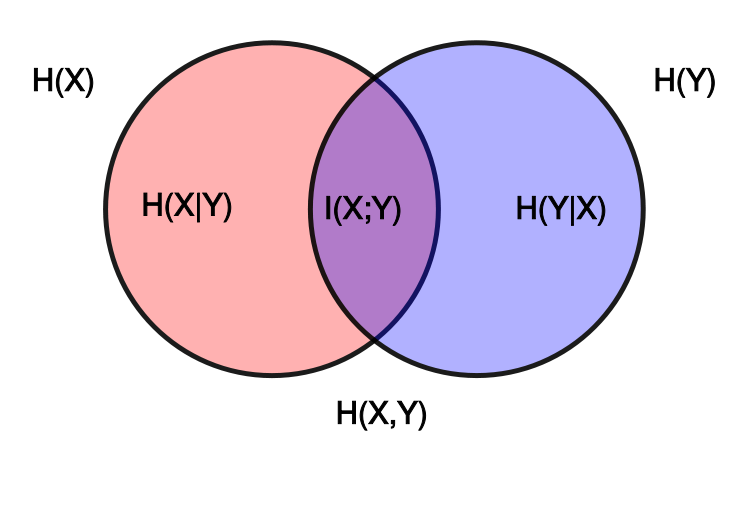
\includegraphics[scale=.25]{mutual-information.png}
\caption{Individual $\mathbb{H}(X),\mathbb{H}(Y)$, joint $\mathbb{H}(X,Y)$, and conditional entropies for a pair of correlated subsystems $X,Y$ with mutual information $\mathbb{I}(X;Y)$.}
\label{fig:mi} 
\end{figure}

Intuitively, we can interpret the MI between $X$ and $Y$ as the reduction in uncertainty about $X$ after observing $Y$, or, by symmetry, the reduction in uncertainty about $Y$ after observing $X$.

A quantity which is closely related to MI is the \textbf{pointwise mutual information} or \textbf{PMI}. For two events (not random variables) $x$ and $y$, this is defined as
\begin{equation}
PMI(x,y) \triangleq \log\dfrac{p(x,y)}{p(x)p(y)}=\log\dfrac{p(x|y)}{p(x)}=\log\dfrac{p(y|x)}{p(y)}
\end{equation}

This measures the discrepancy between these events occuring together compared to what would be expected by chance. Clearly the MI of $X$ and $Y$ is just the expected value of the PMI. Interestingly, we can rewrite the PMI as follows:
\begin{equation}
PMI(x,y)=\log\dfrac{p(x|y)}{p(x)}=\log\dfrac{p(y|x)}{p(y)}
\end{equation}

This is the amount we learn from updating the prior $p(x)$ into the posterior $p(x|y)$ , or equivalently, updating the prior $p(y)$ into the posterior $p(y |x)$ .